\section{Data Collection}
By selecting the measurement devices, namely \gls{imu}s and heart rate \gls{hr} monitors, and specifying state-of-the-art \gls{set}s for each discipline, data collection proceeded by adhering to the prescribed sequence of tasks for each \gls{set}. The subsequent sections provide a more technical description of the biomechanical data collection utilizing the \gls{imu}s and the physiological data acquisition employing \gls{hr} monitors and lactate measurement devices.


\subsection{Biomechanical Data}
For the biomechanical data collection, the horses were equipped with \gls{imu}s. The \gls{imu}s \cite{456} were mounted on the bridle that is fixed on the head between the ears, attached on the skin on the sacrum (tuber sacrale) and withers (in front of the saddle between shoulder blades) using double-sided tape, and placed on customized pockets that were fitted on the lateral side of all four limbs (cannon bone or third metacarpal/metatarsal bone) using hook-and-loop bands. Each \gls{imu} weighed 20 grams. Figure \ref{imuplacementsporthorse} demonstrates the arrangement of \gls{imu}s and their orientations on a sport horse.

\begin{figure}[!htb]
\centering
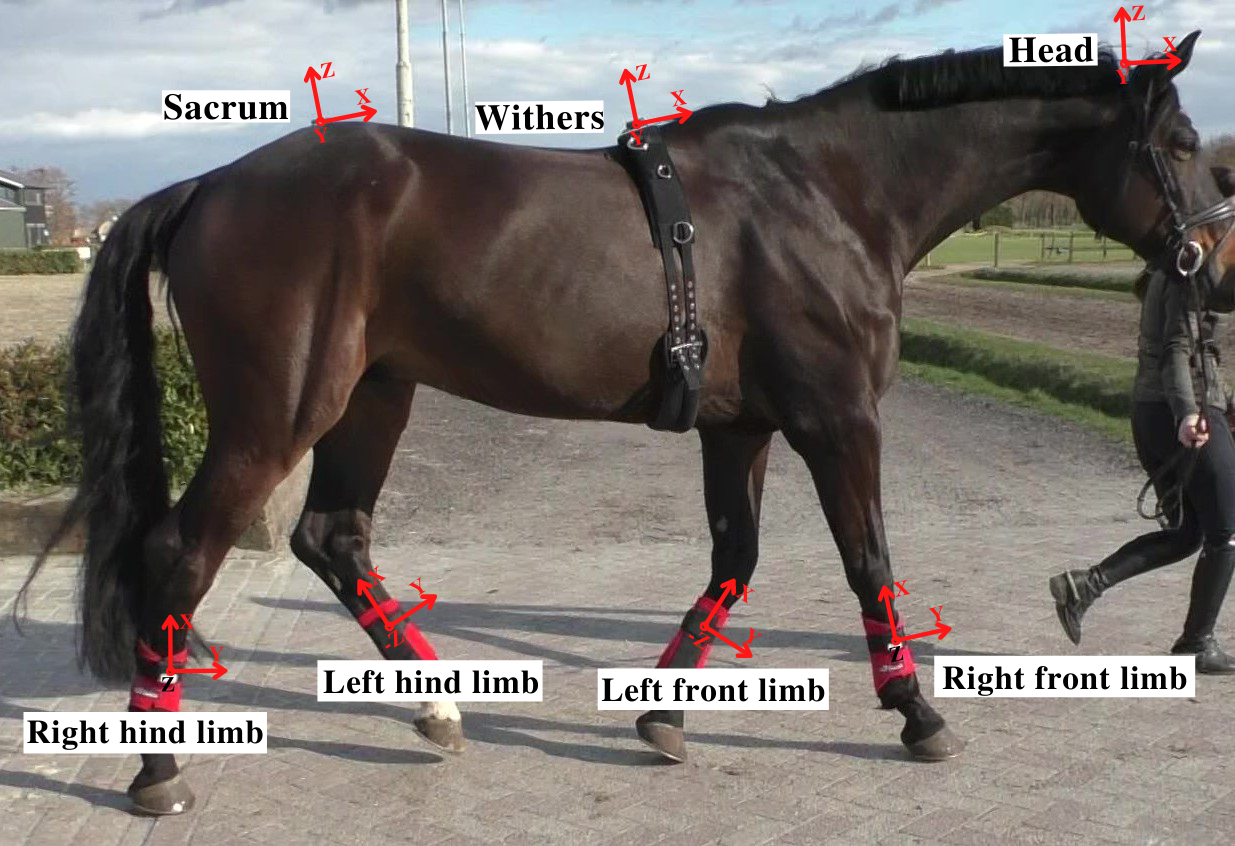
\includegraphics[width=0.95\textwidth]{chapters/data/figures/Sacrum.png}
\caption{{{\gls{imu}s locations and orientations on horse body.} RF: right front limb, LF: left front limb,
RH: right hind limb, LH: left hind limb.}}
\label{imuplacementsporthorse}
\end{figure}

According to Table \ref{tab:IMU info on horses}, the numbers of body-mounted \gls{imu}s were different between horses. The \gls{imu}s contained a tri-axial accelerometer, a tri-axial gyroscope, and a tri-axial magnetometer. The three local axes of the \gls{imu} are presented in Figure \ref{IMUaxes}. Understanding the orientation of local axes facilitates their transformation to a global reference frame to gauge the orientation and displacement of the \gls{imu} in relation to real-world orientations, for example, the measurement of vertical displacement. The accelerometer and the gyroscope were set to a sampling rate of 200 Hz, acceleration range of ± 16 g, and maximum angular velocity of 2000 deg/s. The magnetometer was set to a sampling rate of 100 Hz.

\begin{figure}[!htb]
\centering
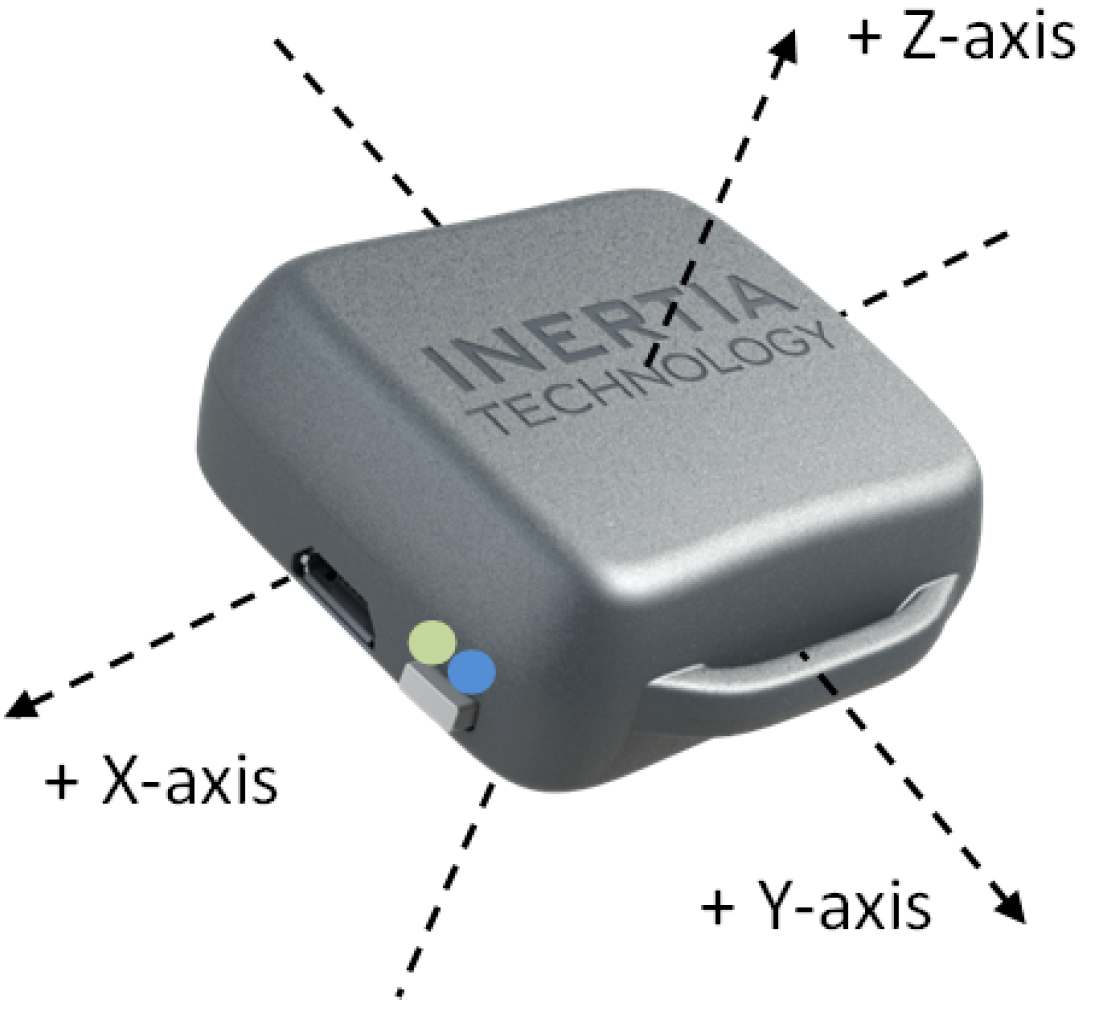
\includegraphics[width=.3\linewidth]{chapters/data/figures/imu.png}
\caption{\gls{imu} local axes. Picture from \cite{a2020_user}}
\label{IMUaxes}
\end{figure}

As demonstrated in Figure \ref{imuplacementsporthorse} and according to the local axes in Figure \ref{IMUaxes}, \gls{imu}s were mounted on the sacrum, withers, and poll in such a manner that their three axes -x, y, and z- are aligned to correspond with the roll, pitch, and yaw angles, respectively. Moreover, the x, y, and z-axis of \gls{imu}s were aligned with internal/external rotation, abduction/adduction, and retraction/protraction of the limbs, respectively. Furthermore, the three axes of horse locomotion, in general, were the longitudinal axis (aligned to the forward locomotion and parallel to the ground), the vertical axis (perpendicular to the ground or parallel to the gravitational force vector), and the mediolateral axis (perpendicular to longitudinal and vertical axes).

\subsection{Physiological Data}
Blood/Plasma \gls{lac} and heart rate were the constituents of collected physiological data. Blood samples were taken from the jugular vein of horses 4 to 5 times during the \gls{set}. The collection of each sample required a duration ranging from 5 to 15 seconds. Then, plasma \gls{lac} was determined using a portable hand-held measurement device (Lactate Pro2, Arkray Inc.). The \gls{hr} was recorded with a sampling frequency of 1 Hz by a heart rate monitor (Polar V800, Polar Electro, Oy, Oulu, Finland) equipped on the horses throughout the \gls{set}.

